\chapter{Umsetzung}

Umgesetzt wurde die Aufgabe im wesentlichen aus drei Teilen: 
\begin{itemize}
	\item Einer SQL-Datenbank mit realitätsnahen Tabellen 
	\item Einer Ontologie 
	\item Einem ausführbaren Programm mit Grafischer Benutzungsoberfläche

\end{itemize}

\section{Datenbank}

Bei der Datenbank wurde auf eine gewöhnliche relationale Datenbank zurückgegriffen, da im wesentlichen nur die gängigsten SQL-Befehle benutzt werden. Da es bereits gute Erfahrungen im Team mit MySQL gab, wurde diese Datenbank verwendet. 

Die Datenbank enthält im wesentlichen Informationen die ein Hochschulsportberater ebenfalls nachschlagen würde. Die wichtigsten Informationen sind:
\begin{itemize}
\item angebotene Sportarten
\item Trainingszeiten
\item Veranstaltungsort
\item Höhe der Teilnehmergebühr
\end{itemize} 

Das genaue Datenbankmodell kann der Abbildung \ref{fig:Datenbank-Design} entnommen werden.

\begin{capfigure}[Datenbank-Design]
	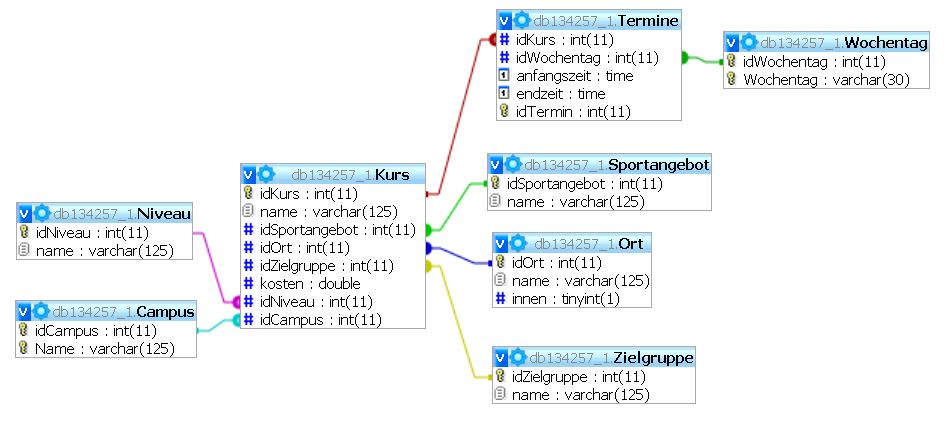
\includegraphics[width=150mm]{images/db_design}
\end{capfigure}

\section{Ontologie}
\TODO{[PRIO:SOFORT] Komplett neu machen}
Die Erstellung der Ontology wird mit \gls{protege} durchgef\"uhrt. \gls{protege} erm\"oglichst nur die Verwendung von OWL-DL. OWL-Full wird nicht unterst\"utzt, daher m\"ussen gewisse Einschr\"ankungen ber\"ucksichtigt werden. Beispielsweise kann man keine Komplementklassen erstellen. 

Desweiteren sollte man immer bedenken, dass eine Ontology ein Open-World-Szenario darstellt. Im speziellen kann man nur nach dem Vorhandensein eines Kriteriums abfragen.

Im Laufe dieses Abschnitts wird erl\"autert, wie die Ontology erstellt wurde. Im Besonderen werden unsere Entscheidungen bei der Umsetzung begr\"undet und deren Folgen erkl\"art.

\subsection{Grobe Unterteilung der Ontology}
Zuerst wird die Klasse \textit{Sport} erstellt. Diese Klasse erh\"alt die beiden Unterklassen \textit{Einzelsport} und \textit{Teamsport}. Da wir uns bei den Sportarten daf\"ur entschieden haben, dass eine Sportart entweder Einzelsport oder Teamsport ist macht diese Unterteilung am meisten Sinn. Nat\"urlich erm\"oglicht diese L\"osung nicht, dass eine Sportart zugleich Einzelsport als auch Teamsport ist. Dies ist aber kein Problem, da es in unserem Szenario nicht vorkommt.

Bei der Darstellung der Ontology lassen wir die Ebene \textit{Thing} aus Gr\"unden der \"Ubersicht weg.
Die Ontology sieht jetzt wie folgt aus:
\begin{capitemize}[Ontology - Grober Unterteilung der Ontology - 1]
		\item Sport
			\begin{itemize}
				\item Einzelsport
				\item Teamsport
			\end{itemize}
\end{capitemize}

Als n\"achstes legen wir die Klassen \textit{Ziele} und \textit{Koerperliche\_Einschraenkungen} an. Diese beiden Klassen dienen dazu die Eigenschaften \textit{Ziele} und \textit{K\"oerperliche Einschr\"ankungen} abzubilden. Beide Klassen werden noch mit den jeweiligen Unterklassen, die die m\"oglichen Optionen darstellen erg\"anzt.

Danach sieht die Ontology wie folgt aus:
\begin{capitemize}[Ontology - Grober Unterteilung der Ontology - 2]
	\item Koerperliche\_Einschraenkungen
		\begin{itemize}
				\item Armbereich
				\item Beinbereich
				\item Hoehenangst
		\end{itemize}
	\item Sport
		\begin{itemize}
			\item Einzelsport
			\item Teamsport
		\end{itemize}
	\item Ziele
		\begin{itemize}
				\item Fitness
				\item Freizeitvergnuegen
				\item SelfDefense
				\item Sozialkontakte
				\item Wettbewerb
		\end{itemize}
\end{capitemize}

Damit sind die Klassen soweit fertig. Beide Klassen wurden in dieser Art angelegt, da sie optional sind. Ein Sport muss keine Verkn\"upfung zu diesen Klassen haben. Jetzt werden noch die Object Properties dazu angelegt. Diese werden wie folgt angelegt:

\begin{capitemize}[Properties - hatZiel und ungeeignetBei]
	\item hatZiel
		\begin{itemize}
			\item Domains: \textit{Sport}
			\item Ranges: \textit{Ziele}
		\end{itemize}
	\item ungeeignetBei
		\begin{itemize}
			\item Domains: \textit{Sport}
			\item Ranges: \textit{Koerperliche\_Einschraenkungen}
		\end{itemize}
\end{capitemize}

Nun lassen sich die Ziele und Einschr\"ankungen mit den Sportarten verbinden. Ein Problem ergibt sich mit dieser Variante allerdings noch, man kann nicht nach Sportarten suchen die keine Einschr\"ankungen haben. Bei den Zielen gibt es die gleiche Einschr\"ankung, allerdings ist sie dort egal, da eine Suche nach Sportarten, die explizit kine Ziele haben keinen Sinn ergibt. Bei den Einschr\"ankungen muss allerdings eine L\"osung her. Da in einem Open-World-Szenario nur nach dem Vorhandensein gefragt werden kann, haben wir uns dazu entschieden noch die Unterklasse \textit{Keine} bei den K\"oerplichen Einschr\"ankungen zu erg\"anzen. Jetzt hat man die M\"oglichkeit auch Sportarten zu suchen, die bei keiner Einschr\"ankung ungeeignet sind.

Bei den Sportarten muss jetzt jede Sportart die Object Property \textit{ungeeignetBei} verwenden. F\"ur die Object Property \textit{hatZiel} gilt das nicht.

\TODO{istExotisch, istKampfsport, istKoerperkontakt, istWassersport - Problem erw\"ahnen, dass man nicht nach Boolean abfragen kann}

\TODO{Klasse Boolean als L\"osung f\"ur das Problem}

\TODO{\"Aquivalenzklassen, Aufbau einer Sportart, etc.}

\section{Programm}

Dieser Abschnitt geht zuerst auf die Entscheidung zum Aufbau der graphischen Oberfläche ein, behandelt danach die technischen Aspekte des Programms und im letzten Teil des Abschnittes wird die Realisierung der Sprünge aus den Szenarien betrachtet. 

\subsection{Entscheidung zum Aufbau der graphischen Oberfläche}
Bei der Gestaltung der GUI, wurde sich dafür entschieden, dass der Benutzer zu jedem Zeitpunkt möglichst alle Auswahlmöglichkeiten vor Augen hat und dass er, ebenfalls zu jedem Zeitpunkt, eine Liste mit den Sportarten erhalten kann, die zu seinen Auswahlkriterien passen.

Die Gründe für diese Entscheidungen sind zum einen die Benutzerfreundlichkeit. Durch diesen Aufbau soll der Benutzer aufgefordert werden, möglichst viele Auswahlkriterien auszuprobieren, da er sofort testen kann, welche Auswirkungen diese auf die Auswahl der Sportarten hat. Dies hat den Vorteil, dass der Benutzer die Kriterien mit, einer für ihn, hohen Priorität setzen kann und unangerührt lässt, währendem er die Kriterien mit einer, für ihn, niedrigen Priorität schnell und einfach ändern kann. Ein konkretes Beispiel hierfür wäre z.B. die Sportart Klettern. Für einige Benutzer ist die Höhenangst nur ein leichtes Problem, für einige andere ist sie unüberwindlich. Somit haben die Benutzer mit leichter Höhenangst, die Möglichkeit die angebotenen Sportarten mit oder ohne Höhenangst zu vergleichen, während jene mit starker Höhenangst das Kriterium auswählen und nicht mehr deaktivieren.

Ein anderer Grund für diese Entscheidung war die Tatsache, dass unsere Szenarien wenige Sprünge von einem Schritt zu einem anderen beinhalten. Deshalb haben wir uns dagegen entschieden eine Frage nach der anderen abzuhandeln, wie die Szenarien dies eigentlich vorsehen und bei mehreren Sprüngen wohl auch einfacher umzusetzen gewesen wäre. Nichtsdestotrotz wird am Ende dieses Abschnittes erläutert wie mehrere dieser Sprünge dargestellt werden könnten, obwohl der Benutzer nach wie vor sämtliche Optionen vor Augen hat und möglichst wenig an Flexibilität einbüßt.

\subsection{Technische Umsetzung}
\TODO{Der Abschnitt ist viel zu detailliert. Das will so niemand lesen. Die prinzipielle Funktionsweise ist wichtig.
Z.B. query (DB, oder Onto) hat immer folgenden Aufbau, Liste query(Liste). Dadurch wird es möglich eine query nach der anderen auszuführen und die Reihenfolge ist auch egal etc... Außerdem viel weniger Code copieren und nicht jedes Detail beschreiben, dies gilt auch für die Screenshots.  }

Das Programm wurde mit Java geschrieben und beinhaltet eine Swing-basierte GUI. Funktional ist sie angebunden an eine SQL-Datenbank und eine OWL-Datei, die die Ontologie repräsentiert. Das Optische Erscheinungsbild ist in zwei Fenster gegliedert: Dem Hauptfenster besehend aus den sechs Auswahlgruppen Art des Sports (Einzel- oder Team), Einem Eingabefenster für maximale Kosten, ein Zielefenster, Innen-Außen-Formular geeignet, Ziele Eigenschaften (Abbildung \ref{GUI1}). Das zweite Fenster ist ein "`Stundenplan"', bei dem durch Auswahl ganzer Tage oder einzelner Stunden im Gitter bei dem die ausgewählten möglichen Zeiträume grün dargestellt werden (Abbildung \ref{GUI2})

\begin{figure}%
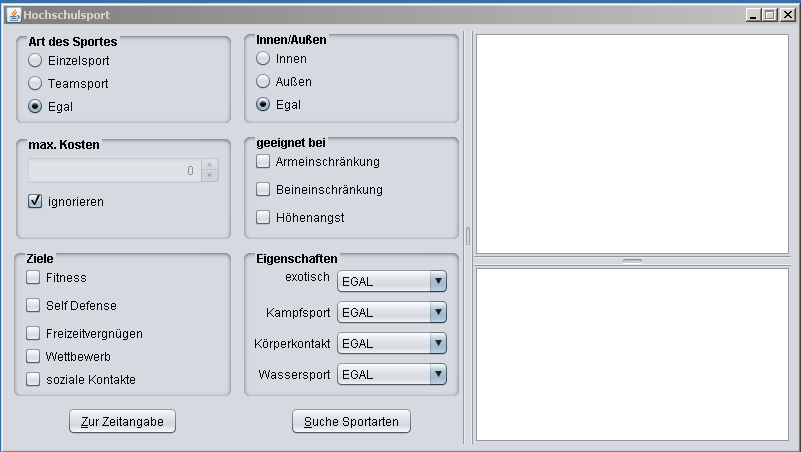
\includegraphics[width=150mm]{images/gui.png}%
\caption{Startpunkt: Die GUI nach Programmaufruf}%
\label{GUI1}%
\end{figure}

\begin{figure}%
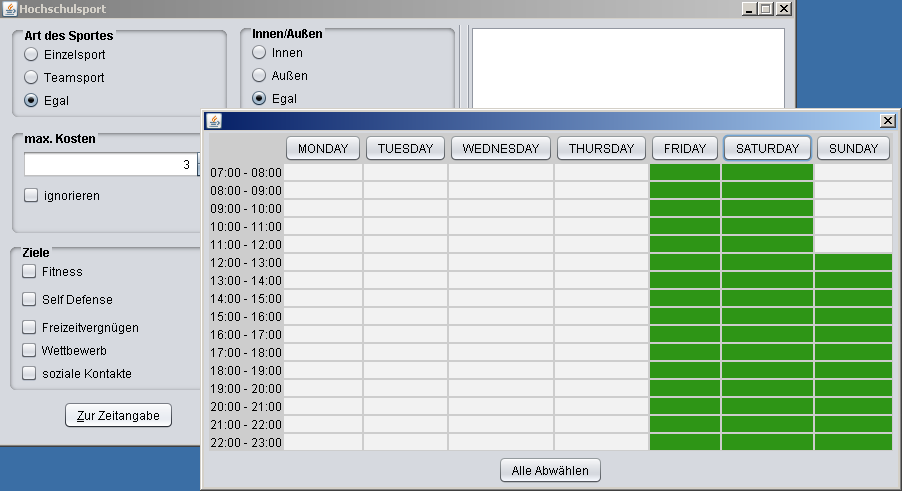
\includegraphics[width=150mm]{images/guizeit.png}%
\caption{Auswahl der Zeiten}%
\label{GUI2}%
\end{figure}

Durch den Knopf "`Suche Sportarten"' wird eine Recherche ausgelöst. Hierfür wird eine Ontologie- und Datenbankverbindung geöffnet.
Die Ontologieverbindung ist durch einen Shortform-Provider aus der OWL-API und einem HermIt-Reasoner realisiert. Letzterem wird über einen Stream unsere OWL-Datei übergeben. Hierfür gibt es die Klasse OntologyConnection, welche als Singleton-Klasse realisiert ist.

Die Datenbankverbindung wird durch einen JDBC-Treiber realisiert. Unsere gefüllte Datenbank liegt auf einem SQL-Server im Internet.

Das folgende Listing wird nach Auslösen des "`Suche Sportarten"'-Knopfes ausgeführt (präziser: Die doInBackground-Methode):


\begin{lstlisting}[language=JAVA]
	private class ExecuteQuery extends SwingWorker<Void, Void> {

		private DefaultListModel<Sportangebot> model = new DefaultListModel<Sportangebot>();
		private QueryBuilder builder;

		@Override
		protected Void doInBackground() throws Exception {
			builder = new QueryBuilder();

			configArtVonSport();
			configPrice();
			configKoerperlicheEinschraenkung();
			configInnenAussen();
			configZiele();
			config4Attributes();
			configTimeFrames();

			Map<String, Sportangebot> result = builder.execute();
			List<Sportangebot> result_sportangebote = new ArrayList<Sportangebot>(
					result.values());
			Collections.sort(result_sportangebote);
			for (Sportangebot sport : result_sportangebote) {
				model.addElement(sport);
			}

			return null;
		}
\end{lstlisting}

Die config-Methoden lesen zunächst die gewählten Optionen aus und bereiten diese für den QueryBuilder derart auf, dass einfach lesbare Datentypen entstehen. Der QueryBuilder gibt eine Menge von Key-Value-Paaren zurück, das aus den gematchten Sportbezeichnungen und der jeweils dazugehörigen Instanz besteht.

Der QueryBuilder führt nun sukzessiv bis zu 8 Queries aus, je nach dem, welche notwendig ist. Als erste die querySport, die alle Sportarten liefert, die sowohl in der Ontologie, als auch in der Datenbank sind. Die zweite Einschränkung käme, wenn Einzel oder Teamsport ausgewählt sind. Bei jeder Ontologie-Einschränkung wird die Query in der Form zusammengebaut: <NEUE QUERY> AND ( jeder Schlüsselwert in sport, getrennt durch OR ). Bei der Datenbank analog mit AND ( Sportangebot.name = 'Sport1' OR Sportangebot.name = 'Sport2' ... ) in der WHERE-Klausel.

Im folgenden 

		


\begin{lstlisting}
    public Map<String, Sportangebot> execute() {
        Map<String, Sportangebot> sport = Queries.querySport();

        if (selectedArtVonSport == ArtVonSport.EINZELSPORT) {
            sport = Queries.queryEinzelsport(sport);
        } else if (selectedArtVonSport == ArtVonSport.TEAMSPORT) {
            sport = Queries.queryTeamsport(sport);
        }

        if (maximalPrice >= 0) {
            sport = Queries.queryPrice(sport, maximalPrice);
        }

        if (einschraenkungen.length > 0) {
            sport = Queries.queryFilterKoerperlicheEinschraenkungen(sport,
                                                                   einschraenkungen);
        }

        if (selectedInnenAussen != InnenAussen.EGAL) {
            boolean indoor = selectedInnenAussen == InnenAussen.INNEN;
            sport = Queries.queryIndoor(sport, indoor);
        }

        if (ziele.length > 0) {
            sport = Queries.queryZiele(sport, ziele);
        }

        if (timeFrames.size() > 0) {
            sport = Queries.queryTimeFrames(sport, getCompactTimeFrames());
        }

        sport = Queries.query4Attributes(sport, kampfsport, exotisch, koerperbetont, wassersport);

        return sport;

    }

\end{lstlisting}

\section{Realisierung der Sprünge}
Da es in unseren Szenarien nur wenige Sprünge gibt, wurde deren Logik fest in die GUI hinein programmiert. Die einzelnen Sprünge sind im folgenden aufgelistet und es wird beschrieben, wie diese umgesetzt wurden.

\subparagraph{Überspringen der Frage ob Einzel- oder Teamsportart.} Der Benutzer kann in der GUI bei dieser Frage "`Egal"' auswählen, so dass sie nicht in Betracht gezogen wird.
\subparagraph{Die Frage ob das Sportangebot etwas kosten darf.} Der Benutzer hat hier die Möglichkeit, die Frage zu ignorieren, oder einen maximal Preis anzugeben.
\subparagraph{Hat der Benutzer eine Einschränkung, so darf beim Sportangebot kein Körperkontakt bestehen.} Wählt der Benutzer eine Einschränkung, so wird die Auswahlmöglichkeit zum Körperkontakt automatisch auf "`Nein"' gestellt und er kann diese Auswahl nicht mehr ändern. Es sei denn er wählt sämtliche Einschränkungen wieder ab.
\subparagraph{Sprung zu einer beliebigen Frage.} Da der Benutzer sämtliche Auswahlkriterien zu jedem Zeitpunkt sehen kann ist dieser Sprung nicht relevant.

\subsection{Realisierung von mehreren Sprüngen}
Diese Vorgehensweise ist recht gut geeignet, falls die Szenarien nur wenige Sprüngen enthalten. Im Falle dass es in diesen mehrere solcher Sprünge gibt, braucht man eine andere Vorgehensweise, bei der diese nicht mehr hartcodiert sind, sondern möglichst dynamisch verändert werden können.

Eine Idee wäre es verschiedene Personenarten in die Ontology einzuführen. Je nach dem welche Angaben der Benutzer ausgewählt hat, ermittelt die Ontology um welche Art von Person es sich beim Benutzer handelt. Die GUI erhält die Personenart und kann entsprechend darauf reagieren, indem sie z.B. verschiedene Felder automatisch auswählt, hervorhebt oder versteckt.

Als Beispiel könnte man eine Personenart \lstinline"eingeschraenkte_Person" in der Ontology einführen, die eine Unterklasse von \lstinline"Person" ist und als Property \lstinline"hat_Einschraenkung some koerperliche_Einschraenkung" besitzt. Wählt der Benutzer nun als körperliche Einschränkung den Beinbreich aus, so wird eine Query an die Ontologie abgesetzt, die wie folgt aussieht \lstinline"Person and hat_Einschraenkung some Beinbereich", das Ergebnis dieser Query wäre die Klasse \lstinline"eingeschraenkte_Person". Da die GUI nun weiß, dass es sich beim Benutzer um eine \lstinline"eingeschraenkte_Person" handelt, kann die Auswahloption der Kampfsportart, wie im Szenario beschrieben, auf \lstinline"Nein" gesetzt werden.

Das Beispiel kann man wie folgt erweitert werden, führt man eine weitere Personenart \lstinline"zahlende_Person" mit der Property \lstinline"will_zahlen only True", wobei es sich bei dem True um einen von uns eingeführten Boolean Wert handelt. Dies ermöglicht es folgende Query abzusetzen: \lstinline"Person and (hat_Einschraenkung some Beinbereich or will_zahlen only True)". Das Ergebnis sind folgende Personenarten: \lstinline"eingeschraenkte_Person, zahlende_Person". Die GUI kann daraufhin auf die einzelnen Personenarten reagieren und wie oben beschrieben ihr Aussehen ändern. Ein Vorteil dieser Methode ist, dass man die Query beliebig mit der Veroderung erweitern kann, so dass man bei Bedarf weitere Kriterien aufnehmen kann.

In diesem Beispiel müssen zwei unabhängige Teile der GUI verändert werden, es ist jedoch vorstellbar, dass es Personenarten gibt, die gleichzeitig auftreten können, allerdings widersprüchliche Effekte in der GUI auslösen sollen. So könnte z.B. ein bestimmtes Feld für die eine Personenart aus- und für die andere Personenart angeschaltet werden. Wie solche Konflikte zu lösen sind, wir wahrscheinlich von den konkreten Fällen abhängen. Ein möglicher Lösungsansatz wäre aber ein Priorisieren der verschiedenen Personenarten. Dies bedeutet, dass sich die Personenart mit der höheren Priorität durchsetzt und die GUI deren Effekte übernimmt. Die Prioritäten könnten auch vom Benutzer mitbestimmt werden, indem er festlegen kann, wie wichtig ihm verschiedene Auswahlkriterien sind.
 














